\documentclass[a4paper,article,14pt]{extarticle}

\usepackage{spbudiploma}
\usepackage{euscript}
\usepackage{longtable}
\usepackage{makecell}
\usepackage[pdftex]{graphicx}
\usepackage{amsthm,amssymb,amsmath}
\usepackage{textcomp}
\usepackage[inkscapeformat=png]{svg}
\usepackage{minted} % требует параметра -shell-escape
\usepackage[ruled]{algorithm2e}

\usepackage{tabularx}
\usepackage{booktabs}
\renewcommand{\arraystretch}{1.2}

\renewcommand{\theFancyVerbLine}{\sffamily{\small \oldstylenums{\arabic{FancyVerbLine}}}}

\newenvironment{code}[1]{
  \VerbatimEnvironment
  \begin{minipage}{3cm}
  \vspace*{+1em}
  \begin{minted}[linenos,baselinestretch=1,style=abap]{#1}}{
  \end{minted}
  \vspace*{+0.3em}
  \end{minipage}
}

\newenvironment{codenl}[1]{ % no lines
  \VerbatimEnvironment
  \begin{minipage}{3cm}
  \vspace*{+1em}
  \begin{minted}[style=abap]{#1}}{
  \end{minted}
  \vspace*{+0.3em}
  \end{minipage}
}

\newenvironment{zerocode}[1]{
  \VerbatimEnvironment
  \begin{minipage}{3cm}
  \vspace*{+1em}
  \begin{minted}[baselinestretch=1,style=abap]{#1}}{
  \end{minted}
  \vspace*{+0.3em}
  \end{minipage}
}

\newenvironment{nocode}{
  \VerbatimEnvironment
  \begin{minipage}{3cm}
  \vspace*{+1em}
  \begin{minted}[baselinestretch=1]{yaml}}{
  \end{minted}
  \vspace*{+0.3em}
  \end{minipage}
}

\newcommand{\var}[1]{$\mathtt{#1}$}

\begin{document}

\newgeometry{left=30mm, top=20mm, right=15mm, bottom=20mm, nohead, nofoot}
\begin{titlepage}
\begin{center}

% \textbf{Санкт--Петербургский государственный университет}\\
% \textbf{Факультет математики и компьютерных наук}
Санкт--Петербургский государственный университет


\vspace{35mm}

\textbf{\textit{\large Строганов Никита Сергеевич}} \\[8mm]
\textbf{\large Выпускная квалификационная работа}\\[3mm]
\textbf{\textit{\large Разработка инструмента для автоматического обнаружения архитектурных антипаттернов в микросервисных системах}}

\vspace{20mm}
Уровень образования: магистратура\\
Направление 01.04.02 «Прикладная математика и информатика»\\
Основная образовательная программа ВМ.5889.2023\\
«Разработка программного обеспечения и науки о данных»\\
Профиль Архитектура больших систем\\[20mm]
\end{center}

\begin{flushright}
\begin{minipage}[t]{0.65\textwidth}
% \begin{minipage}[t]{0.72\textwidth}
{Научный руководитель:} \\
доцент, факультет математики и компьютерных наук СПбГУ, к.ф.-м.н., Д.С.\,Шалымов
\vspace{10mm}
% \vspace{6mm}

% {Консультант:} \\
% руководитель службы, ООО «Яндекс.Вертикали Технологии», М.\,Чугунков
% \vspace{6mm}

{Рецензент:} \\
разработчик, ООО «Яндекс.Вертикали Технологии», А.В.\,Тараскин
\end{minipage}
\end{flushright}

\vfill

\begin{center}
{Санкт-Петербург}
\par{\the\year{} г.}
\end{center}
\end{titlepage}
\restoregeometry
\addtocounter{page}{1}


\tableofcontents
\pagebreak

\specialsection{Введение}

Современные микросервисные системы состоят из десятков и даже сотен компонентов, каждый из которых решает узкоспециализированную задачу и взаимодействует с другими через чётко определённые интерфейсы \cite{msa-overview}. Такой архитектурный подход обеспечивает масштабируемость, отказоустойчивость и модульность, однако одновременно с этим он порождает значительные сложности. В частности, становится всё труднее поддерживать целостность системы и соблюдать архитектурные решения, принятые на этапе проектирования. В отличие от ошибок в программной логике, архитектурные нарушения, как правило, не приводят к немедленным сбоям, но накапливаются в виде технического долга. Это снижает сопровождаемость системы, тормозит развитие и в перспективе ведёт к ухудшению качества продукта \cite{arch-debt}.

Процесс проектирования архитектуры включает в себя множество артефактов: диаграммы зависимостей, схемы взаимодействия, текстовые описания и негласные договорённости между командами. Эти материалы описывают желаемую структуру системы, однако со временем неизбежно устаревают и перестают отражать её фактическое состояние. При этом визуальные схемы или текстовые спецификации по своей природе носят декларативный характер — они позволяют понять, как компоненты связаны в идеале, но не дают ответа на вопрос, какие связи действительно реализованы в коде или конфигурациях. Например, архитектор может задать, что все интеграции с внешним сервисом должны проходить через слой Anti-Corruption Layer (ACL) \cite{acl-pattern}, однако у него нет надёжного способа проконтролировать соблюдение этого правила. Через некоторое время в систему может быть добавлена прямая зависимость от внешнего сервиса, нарушающая принцип изоляции, — и это останется незамеченным.

Подобные сценарии подчёркивают ключевую проблему: наличие формальных архитектурных принципов не гарантирует их соблюдение на практике. Архитектору сложно контролировать реализацию даже собственных решений, особенно когда архитектурные нарушения не приводят к очевидным ошибкам на уровне бизнес-логики. Ещё сложнее — количественно оценить архитектурный техдолг проекта. Между тем, эта метрика может быть крайне важной как для архитекторов, так и для разработчиков. Например, если в системе насчитывается пять случаев совместного доступа нескольких сервисов к одной и той же базе данных (антипаттерн shared-database \cite{antipatterns-taxonomy}), это является объективным показателем архитектурных нарушений. После проведения рефакторинга и устранения части таких связей можно говорить об <<измеримом>> улучшении архитектуры, опираясь на описанную метрику. Рост этой метрики, напротив, может сигнализировать о нарастающей деградации архитектуры, даже если это пока не отражается на функциональности приложения.

Один из подходов, частично решающий проблему документирования и контроля архитектуры, — это инфраструктура как код (Infrastructure-as-Code, IaC \cite{iac-concept}). В рамках него сервисы, базы данных и другие элементы окружения описываются в виде конфигураций, хранимых в системах контроля версий и проходящих те же процедуры ревью, что и программный код. Это позволяет воспроизводимо разворачивать окружение, отслеживать изменения и минимизировать влияние человеческого фактора. Более того, IaC обеспечивает явную связь между кодом и его инфраструктурным контекстом, снижая риск несогласованности. Однако даже в условиях, когда всё окружение формально описано, смысл архитектурных решений и бизнес-ограничений по-прежнему анализируется вручную.

Существующие инструменты, такие как ArchUnit, SonarGraph и некоторые другие, в определённой степени предоставляют поддержку автоматизированной валидации архитектурных ограничений. Они позволяют описывать правила с помощью собственных DSL-языков и применять проверки на соответствие этим правилам \cite{dsl-fowler}. Однако на практике эти решения нередко оказываются слишком ограниченными или сложными в интеграции. Высокий порог входа, необходимость точной настройки и ограниченная выразительность часто делают их неудобными для использования во времена быстрой эволюции микросервисных систем — особенно при наличии особенностей окружения, специфичных для конкретной организации. Более того, подавляющее большинство этих инструментов не предоставляют агрегированного представления архитектурного состояния, не поддерживают визуализацию отклонений и почти не используют числовые метрики, которые могли бы помочь в анализе архитектурного долга и его динамики во времени.

Таким образом, существует потребность в инструменте, который бы позволял явно описывать архитектурные принципы системы и проверять их соблюдение автоматически. При этом важно, чтобы такой инструмент был удобен для использования в процессе разработки: позволял быстро формулировать правила любой сложности, удобно запускался и органично интегрировался в инфраструктуру компании.

Данная работа направлена на анализ обозначенной проблемы и разработку подхода, позволяющего автоматически выявлять архитектурные антипаттерны в микросервисных системах. Основной акцент делается на практическую применимость, гибкость расширения набора проверок и удобство использования инструмента в рамках жизненного цикла разработки. Результатом станет прототип системы, способной на основе инфраструктурных конфигураций и связей между сервисами выявлять потенциальные архитектурные нарушения и тем самым способствовать контролю качества архитектуры в условиях её неизбежной эволюции.

Практическая реализация и апробация предлагаемого в данной работе инструмента будут проводиться в инфраструктуре Яндекс.Вертикалей. Это означает, что разрабатываемое решение будет изначально ориентировано на интеграцию с существующими в компании системами управления конфигурациями и развертывания. Такой подход позволит проверить инструмент на реальных задачах и сфокусироваться на решении архитектурных проблем, наиболее актуальных для компании, с учетом специфики технологического стека.

\specialsection{Постановка задачи}

Целью данной работы является разработка инструмента, который бы позволил автоматически проверять архитектуру микросервисной системы на соответствие заложенным в неё принципам. Для достижения цели были сформулированы следующие задачи.

\begin{itemize}
    \item Провести обзор предметной области и подходов существующих анализаторов с целью выявления их достоинств и недостатков.
    \item Разработать инструмент, позволяющий описывать правила любой сложности и проверять их выполнение применимо к конкретной архитектуре.
    \item Придумать простой способ написания новых правил для шаблонных ситуаций.
    \item Предоставить правила, проверяющие соблюдение стандартных архитектурных антипаттернов, и заложить их в инструмент по умолчанию.
    \item Проинтегрировать решение с используемыми в Яндекс.Вертикалях системами и инструментами разработки.
    \item Измерить эффективность и полезность инструмента на реальных микросервисных системах, а также проанализировать полученные результаты.
\end{itemize}

\section{Обзор предметной области}

Одним из ключевых аспектов, влияющих на долгосрочную жизнеспособность и эффективность микросервисных систем, является качество их архитектуры. Принятые на этапе проектирования решения определяют, насколько система будет гибкой, масштабируемой, отказоустойчивой и простой в сопровождении. Однако, как было отмечено во введении, существует значительный разрыв между декларируемыми архитектурными принципами и их фактической реализацией. Этот разрыв часто приводит к появлению так называемых архитектурных антипаттернов.

\subsection{Архитектурные антипаттерны}

Архитектурные антипаттерны — это неэффективные или неудачные решения повторяющихся проблем проектирования программных систем. Подобно тому, как <<паттерны проектирования>> предлагают проверенные временем решения для типичных задач \cite{microservices-patterns}, антипаттерны описывают распространённые ошибки и <<ловушки>>, в которые легко попасть при разработке. Возникновение антипаттернов часто является следствием неполного понимания проблемы, ограниченности ресурсов, давления сроков, недостаточной коммуникации между командами или постепенной эрозии первоначального замысла под влиянием изменений и доработок. Антипаттерны могут приводить к увеличению сложности, снижению производительности железа или к затруднению дальнейшего развития системы \cite{antipattern-def}.

Для более глубокого понимания проблемы рассмотрим буквально два известных примера архитектурных антипаттернов.

\subsubsection{Shared Database}

Одним из наиболее известных и часто встречаемых антипаттернов в микросервисных системах является <<Общая база данных>> (Shared Database \cite{shared-db-ap}). Он возникает, когда несколько независимых микросервисов напрямую обращаются к одной и той же физической базе данных, используя общие таблицы или даже всю схему данных. На первый взгляд, такое решение может показаться удобным, особенно на ранних этапах разработки или при миграции от монолитной архитектуры, поскольку оно упрощает обмен данными и позволяет избежать дублирования. Однако в долгосрочной перспективе общая база данных становится источником множества проблем.

\begin{figure}[ht]
   \centering
   \includesvg[scale=1]{images/shared-database.drawio.svg}
   \caption{\label{shared-database} Пример антипаттерна Shared Database.}
\end{figure}

Во-первых, она создаёт сильную связанность между сервисами на уровне данных. Любое изменение схемы базы данных, инициированное одним сервисом (например, добавление нового поля, изменение типа данных или удаление таблицы), может немедленно повлиять на работоспособность других сервисов, использующих эту же схему. Это приводит к тому, что команды разработки становятся зависимыми друг от друга, а процесс внесения изменений усложняется и требует тщательной координации, что противоречит идее автономности микросервисов.
Во-вторых, общая база данных затрудняет независимое масштабирование сервисов. Если один из сервисов создаёт высокую нагрузку на базу данных, это неизбежно скажется на производительности всех остальных сервисов, которые от неё зависят. База данных становится <<узким горлышком>> и единой точкой отказа для целой группы сервисов.
В-третьих, нарушается принцип инкапсуляции данных. Каждый микросервис должен владеть своими данными и предоставлять доступ к ним исключительно через чётко определённый API \cite{data-encapsulation-msa}. Прямой доступ к данным другого сервиса в обход его API нарушает этот принцип, делая систему более хрупкой и сложной для понимания.

% \subsubsection{God Service}

% Другим распространённым антипаттерном является <<Божественный сервис>> (God Service) или <<микромонолит>>. Этот антипаттерн характеризуется наличием сервиса, который аккумулируют слишком много разнородных функций и знаний о других частях системы. Такой сервис становится центральным узлом, через который проходит большинство взаимодействий, и он часто знает о деталях реализации других сервисов, с которыми интегрируется.
% Проблема микромонолита заключается в том, что он нарушает принцип единой ответственности и приводит к тем же недостаткам, которые присущи монолитным архитектурам, но теперь уже на уровне отдельного сервиса. Разработка и тестирование такого сервиса усложняются из-за его большого размера и множества зависимостей. Любые изменения в нём потенциально затрагивают значительную часть функциональности системы, что увеличивает риски при развёртывании. Масштабирование такого сервиса также становится неэффективным, поскольку приходится масштабировать все его функции целиком, даже если высокая нагрузка возникает только на одной из них. Более того, отказ <<божественного сервиса>> может привести к каскадному отказу значительной части системы, снижая её общую отказоустойчивость.
% Возникновение такого антипаттерна часто связано с постепенным разрастанием функциональности существующего сервиса, когда новые задачи добавляются в наиболее подходящий с точки зрения текущего контекста сервис, не задумываясь о долгосрочных архитектурных последствиях.

\subsubsection{Lava Flow}

Следующий пример антипаттерна, иллюстрирующий сложности поддержания архитектурной целостности, – это <<Поток лавы>> (Lava Flow \cite{lava-flow-ap}). Этот антипаттерн описывает ситуацию, когда в системе накапливаются устаревшие компоненты или код, которые никто не решается удалить из-за страха нарушить работоспособность системы. Оставаясь в системе, они затрудняют её понимание, сопровождение и развитие.
<<Поток лавы>> может проявляться в виде мёртвого кода, неиспользуемых конфигурационных параметров или даже целых сервисов и баз данных, которые когда-то были нужны, но со временем их функциональность была перенесена или стала ненужной. Проблема заключается в том, что наличие таких артефактов увеличивает когнитивную нагрузку на разработчиков и архитекторов. Приходится тратить время на анализ этих элементов, чтобы понять, нужны ли они ещё, и как они взаимодействуют (или не взаимодействуют) с остальной системой. Это замедляет разработку новых функций и увеличивает риск внесения ошибок.
Сложность борьбы с описанным антипаттерном заключается в отсутствии точной информации о реальном использовании тех или иных частей системы. Документация часто отстаёт от реального положения дел, а разработчики, которые изначально создавали эти компоненты, могли уже покинуть проект. В результате, решение об удалении чего-либо принимается с большой осторожностью, и часто проще оставить всё как есть, усугубляя проблему.

\subsection{Существующие инструменты}

Ключевая проблема, которую подчёркивают архитектурные антипаттерны, заключается в том, что их возникновение часто является постепенным и незаметным процессом. В больших, динамично развивающихся микросервисных системах архитектору чрезвычайно сложно отслеживать соблюдение всех заложенных принципов вручную. Архитектурные диаграммы и описания показывают желаемое состояние, но не гарантируют его реализацию. Эта ситуация породила спрос на инструменты, способные автоматически анализировать фактическую структуру системы и выявлять отклонения от заданных архитектурных правил. Рассмотрим некоторые из существующих подходов и инструментов.

\subsubsection{ArchUnit}

ArchUnit представляет собой бесплатную библиотеку с открытым исходным кодом для языка Java, предназначенную для проверки архитектурных правил непосредственно в коде \cite{archunit-site}. Она позволяет разработчикам писать модульные тесты, которые анализируют байт-код приложения и проверяют его на соответствие заданным ограничениям. Правила описываются с помощью гибкого и выразительного предметно-ориентированного языка (DSL).

Например, можно легко определить правило, запрещающее классам из доменного слоя (\verb|..domain..|) зависеть от классов слоя представления (\verb|..web..|), или более сложные правила, описывающие слоистую архитектуру и разрешённые зависимости между ними:

\begin{code}{java}
class ArchitectureTest {
    private final ClassFileImporter importer = 
            new ClassFileImporter();
    private final JavaClasses importedClasses =
            importer.importPackages("com.example");

    @Test
    void domainModelDoesNotDependOnUpperLayers() {
        ArchRule rule = noClasses()
                .that().resideInAPackage("..domain..")
                .should().dependOnClassesThat()
                .resideInAnyPackage("..web..");

        rule.check(importedClasses);
    }
}
\end{code}

Сильной стороной ArchUnit является его интеграция в процесс непрерывной интеграции (CI/CD), где архитектурные тесты выполняются наряду с другими автоматизированными тестами, предотвращая попадание нарушений в основную кодовую базу. Однако ArchUnit ориентирован исключительно на анализ архитектуры внутри одного Java-приложения (монолита или отдельного микросервиса), и не предназначен для анализа межсервисных взаимодействий.

\subsubsection{SonarGraph и Structure101}

Инструменты SonarGraph (часть коммерческой платформы SonarQube \cite{sonargraph-tool}) и Structure101 \cite{structure101-tool}, фокусируются на визуализации и анализе зависимостей на более высоком уровне абстракции – между модулями или компонентами системы.

SonarGraph позволяет архитекторам определять эталонную архитектуру, описывая компоненты системы и разрешённые зависимости между ними. Затем, в процессе анализа кода, SonarGraph сопоставляет фактические зависимости с этой моделью и сообщает о нарушениях. Например, архитектор может задать правило, что модуль \verb|ServiceA| не должен напрямую обращаться к модулю \verb|ServiceB|, а только через общий модуль \verb|CoreServices|. При обнаружении прямого вызова SonarGraph отметит это как нарушение. Инструмент интегрируется в SonarQube и помогает отслеживать соответствие архитектурным гайдлайнам в динамике.

Structure101 предоставляет средства для визуализации архитектуры. Он строит диаграммы зависимостей, которые помогают выявлять запутанные узлы системы, циклические зависимости и чрезмерно крупные компоненты. Structure101 использует метрики для количественной оценки степени нарушения архитектурных принципов (например, принципа единой ответственности на уровне компонентов). На основе этих данных разработчики могут анализировать архитектуру и принимать решения о рефакторинге. Однако никакой автоматизации в этом месте инструмент не предоставляет.

Эти инструменты полезны для получения общего представления об архитектуре. Однако их практическое применение может быть сопряжено с трудностями. Создание и поддержка актуальной архитектурной модели для сложной, быстро меняющейся микросервисной системы требует значительных усилий. Встроенные языки для описания правил могут оказаться недостаточно гибкими для формализации всех специфических требований проекта. Кроме того, основной фокус этих инструментов – анализ кода, и им может не хватать информации о связях, определённых на уровне инфраструктуры.

\subsubsection{Концепция тестов на архитектуру}

Наиболее близким по идеологии к задачам данной работы является подход, представленный в докладе <<Раз архитектура — "as Code"\text{,} почему бы её не покрыть тестами?!>> на конференции ArchDays 2023 \cite{archdays-talk-aac}.

Центральная идея этого подхода заключается в активном использовании артефактов, создаваемых в рамках практик <<Infrastructure-as-Code>> (IaC) и <<Architecture-as-Code>> (AaC). Если инфраструктура системы (сервисы, базы данных, сетевые настройки) описывается в виде кода (например, с помощью Terraform \cite{terraform}, Kubernetes manifests \cite{k8s-manifests}, Ansible \cite{ansible} и так далее), а архитектурные диаграммы и модели также хранятся в текстовом, машиночитаемом формате (PlantUML \cite{plantuml-tool}, Mermaid \cite{mermaid-tool}), то появляется возможность для их автоматического сопоставления и анализа. Примеры IaC-конфигурации и AaC-диаграмы приведены в листингах \ref{iac-example} и \ref{aac-example}.

\begin{listing}[ht]
\begin{codenl}{terraform}
    resource "docker_container" "service_b" {
      name  = "service-b"
      image = "myregistry/service-b:latest"
      ports {
        internal = 8081
        external = 8081
      }
      env = [
        "DATABASE_URL=postgresql://database-b:5432/mydb"
      ]
    }    
\end{codenl}
\caption{Пример простой Terraform-конфигурации.}
\label{iac-example}
\end{listing}

\begin{listing}[ht]
\begin{codenl}{text}
    @startuml C4ContainerDiagram
    
    Container_Boundary(boundary, "System") {
        Container(serviceA, "ServiceA")
        Container(serviceB, "ServiceB")
        ContainerDb(databaseB, "DatabaseB")
    }
    
    Rel(serviceA, serviceB, "Calls", "HTTP/REST")
    Rel(serviceB, databaseB, "Reads/Writes", "JDBC")
    
    @enduml
\end{codenl}
\caption{Пример PlantUML-диаграммы в формате C4 Model.}
\label{aac-example}
\end{listing}

Концепция <<Архитектура как тесты>> предлагает решать две фундаментальные проблемы, свойственные традиционному управлению архитектурой. Во-первых, это проблема устаревания архитектурной документации. В динамично развивающихся системах любые изменения в реальной конфигурации сервисов или их взаимодействий должны немедленно отражаться в архитектурных схемах. В противном случае документация быстро теряет свою актуальность и перестаёт быть надёжным источником информации. Предлагаемый подход позволяет автоматически сравнивать реальную конфигурацию, извлечённую из IaC-артефактов, с задокументированной архитектурой из AaC-источников. Любое расхождение выявляется при прогоне тестов в CI/CD пайплайне, сигнализируя о необходимости либо обновить документацию, либо откатить несогласованное изменение в инфраструктуре. Таким образом, обеспечивается синхронизация реального состояния системы с её описанием.

Во-вторых, решается проблема декларативности и неявности архитектурных ограничений в схемах. Сами по себе диаграммы часто показывают лишь существующие связи, но не отвечают на вопрос, какие связи запрещены или какие архитектурные принципы должны соблюдаться. Например, если на диаграмме \verb|ServiceA| не взаимодействует напрямую с базой данных сервиса \verb|ServiceB|, то неясно, можно ли в будущем добавить такую связь или нельзя. Архитектура в виде картинки об этом ничего не говорит (рис. \ref{declarative-example}).

\begin{figure}[ht]
   \centering
   \includesvg[scale=1]{images/declarative-example.drawio.svg}
   \caption{\label{declarative-example} Декларативность архитектурных диаграмм.}
\end{figure}

Подход <<Архитектура как тесты>> позволяет формализовать эти неявные правила и принципы в виде исполняемых тестов. Эти тесты оперируют графом зависимостей, построенным на основе архитектурных диаграмм AaC. Таким образом, становится возможным валидировать архитектурные решения, заложенные именно в этих диаграммах. Например, можно написать тест, проверяющий, что ни один сервис, кроме \verb|ServiceB|, не зависит от \verb|DatabaseB|, и этот тест будет выполняться на модели, извлечённой из PlantUML-описания.

Прототип инструмента, предлагаемый в рамках этой концепции, включает автоматический парсинг IaC-конфигураций для получения графа реальных связей и AaC-диаграмм для получения графа ожидаемых или эталонных связей. Далее, с помощью набора обычных unit-тестов, производится проверка различных свойств этих графов. Это могут быть тесты на полное соответствие двух графов, тесты на отсутствие определённых типов связей в реальной архитектуре, если они не разрешены в эталонной, или тесты, проверяющие соблюдение высокоуровневых архитектурных принципов.

Для лучшего понимания подхода рассмотрим пример теста, который проверяется, что только сервисы, помеченные тегом \verb|"acl"|, могут иметь зависимости от внешних систем:

\begin{code}{javascript}
it("only acl can depence from external systems", () => {
  let violationsCount = 0;

  for (const container of containersFromPuml) { 
    const isAcl = container.tags?.includes("acl");
    const externalRelations = container.relations.filter(
      (relation) => relation.to.type === ExternalType
    );
    
    if (!isAcl && externalRelations.length > 0) {
      violationsCount += externalRelations.length;
    }
  }

  expect(violationsCount).toBe(0); 
});
\end{code}

Интеграция таких тестов в CI/CD-конвейер позволяет превратить архитектурные принципы из деклараций в исполняемые спецификации. Любое изменение, нарушающее эти принципы или приводящее к рассинхронизации с документацией, будет автоматически обнаружено. Единственное серьёзное ограничение данного подхода — наличие внедренной в компании практики Architecture-as-Сode. Также важно отметить, что рассмотренный инструмент находится на стадии прототипа, то есть скорее демонстрирует интересную идею, чем предоставляет готовое к использованию решение.

\subsubsection{Выводы}

Проведённый обзор существующих решений для контроля архитектуры показывает, что многие из них имеют значительные недостатки или недоработки, препятствующие их практическому применению на реальных микросервисных системах. Так ArchUnit ориентирован на анализ кода только внутри одного сервиса. SonarGraph и Structure101 не предоставляют никакой автоматизации для проверки соблюдения принципов. Концепция <<Архитектура как тесты>> пока что находится на стадии прототипа, а также требует наличие в проекте архитектурных диаграмм в виде кода, что на самом деле является серьезным ограничением. Также стоит отметить, что все рассмотренные подходы требуют усилий по интеграции с корпоративными решениями, инструментами разработки и инфраструктурой.

\newpage

\subsection{Инфраструктура как код}

Концепция Infrastructure-as-Code (IaC) представляет собой подход к управлению и предоставлению вычислительной инфраструктуры (серверов, сетей, хранилищ, балансировщиков нагрузки, баз данных и других компонентов) через машиночитаемые файлы определений, а не посредством ручной настройки или интерактивных инструментов конфигурирования. Эти файлы, вместе с исходным кодом самих сервисов, хранятся в системе контроля версий, проходят через процессы ревью и автоматизированного развёртывания. Такой подход существенно упрощает внедрение и сопровождения IT-инфраструктуры, особенно в контексте облачных вычислений и микросервисных архитектур.

Основными принципами IaC являются автоматизация, воспроизводимость и идемпотентность \cite{iac-principles}. Автоматизация достигается за счёт использования специализированных инструментов, которые интерпретируют файлы определений и приводят инфраструктуру в желаемое состояние. Воспроизводимость означает, что одна и та же конфигурация, применённая в различных окружениях, будет создавать идентичные или предсказуемо схожие инфраструктурные ландшафты. Идемпотентность гарантирует, что повторное применение одной и той же конфигурации не приведёт к нежелательным изменениям, если система уже находится в целевом состоянии.

Существует множество инструментов, реализующих подход IaC: AWS CloudFormation, Terraform, Azure Resource Manager templates, Google Cloud Deployment Manager, Ansible, Puppet, Chef и многие другие. Эти инструменты позволяют описывать желаемое состояние инфраструктуры, используя либо декларативный (описание конечного результата), либо императивный (описание последовательности шагов для достижения результата) стиль. Например, в Terraform разработчик описывает ресурсы (виртуальные машины, базы данных, сетевые правила) и их взаимосвязи в текстовых файлах \verb|.tf|. Terraform затем вычисляет план действий для создания или изменения инфраструктуры до соответствия этому описанию. Аналогично, манифесты Kubernetes в формате YAML или JSON описывают развёртывания, сервисы, конфигурационные карты и другие сущности, необходимые для запуска приложений в контейнерах.

Таким образом, IaC-артефакты представляют собой формализованное и машиночитаемое описание инфраструктуры, где определяются структурные зависимости и связи между компонентами системы:

\begin{itemize}
    \item Определения взаимосвязей ресурсов. IaC-инструменты описывают не только сами компоненты, но и то, как они связаны. Например, Terraform-конфигурация может явно указывать, что определённый микросервис использует конкретный экземпляр базы данных, передавая его адрес через переменные окружения.
    \item Service Mesh. инструменты типа Istio или Linkerd, управляемые через IaC-манифесты, содержат детальные политики взаимодействия между сервисами \cite{istio-mesh}.
    \item Сетевые конфигурации. Правила файрволов, группы безопасности и так далее явно разрешают или запрещают коммуникацию между определёнными IP-адресами или группами ресурсов.
\end{itemize}

Анализ этих конфигурационных файлов позволяет построить граф реальных зависимостей системы. Этот граф отражает, как сервисы связаны друг с другом, какие общие ресурсы они используют, и какие коммуникационные пути между ними фактически настроены. Полученная модель может быть использована для анализа, направленного на выявление архитектурных антипаттернов. Правда, здесь необходимо отметить, что IaC не способен составить архитектурную модель верную на 100\%. В частности, динамические связи, устанавливаемые непосредственно в коде приложений во время выполнения, могут оставаться невидимыми. Однако такой подход сам по себе является в некотором роде <<антипаттерном>>, и обычно разработчики стараются выносить зависимости между сервисами на уровень конфигурации.

\subsection{Система деплоя Shiva}

В контексте разработки инструмента для автоматического обнаружения архитектурных антипаттернов в Яндекс.Вертикалях, ключевым источником информации о фактической структуре системы и связях между её компонентами выступает внутренняя система управления деплоями — Shiva. Shiva представляет собой инфраструктурный сервис, который абстрагирует разработчиков от деталей оркестрации контейнеров и механизмов service discovery, предоставляя унифицированный интерфейс для развёртывания и управления жизненным циклом микросервисов.

Центральным артефактом, с которым работает Shiva, является <<карта сервиса>> (service map). Это декларативное описание сервиса в формате YAML, содержащее всю необходимую метаинформацию. Карта сервиса включает в себя:

\begin{itemize}
    \item \verb|name|: Уникальное имя сервиса.
    \item \verb|type|: Тип компонента (например, \verb|service|).
    \item \verb|owners|: Список ответственных за сервис команд.
    \item \verb|provides|: Определяет интерфейсы, которые сервис предоставляет другим компонентам. Каждый такой интерфейс описывается именем, протоколом, портом и некоторыми другим опциональными параметрами.
    \item \verb|depends_on|: Список сервисов, от которых зависит данный компонент. Для каждой зависимости указывается имя целевого сервиса (\verb|service_name|) и имя используемого интерфейса (\verb|interface_name|). На данный момент секция не является обязательной, поэтому для большинства сервисов все их реальные зависимости не будут отражены в этом списке.
\end{itemize}

А также многие другие поля, менее важные в контексте составления графа зависимостей. Ниже приведен простейший пример карты сервиса в Shiva:

\begin{nocode}
name: service-a
type: service
provides:
- name: grpc-api
  protocol: grpc
  port: 80
depends_on:
- service_name: service-b
  interface_name: http-api
\end{nocode}

На основе карты сервиса Shiva подготавливает инфраструктуру для контейнеров, управляет их ресурсами и жизненным циклом. Процесс деплоя также конфигурируется декларативно с помощью манифеста деплоя, который является ещё одним YAML-файлом. Манифест деплоя определяет параметры развёртывания для различных окружений (prod и test), включая:

\begin{itemize}
    \item \verb|datacenters|: Количество инстансов сервиса в каждом дата-центре.
    \item \verb|resources|: Запросы к ресурсам (CPU, память).
    \item \verb|config|: Специфичные для окружения конфигурации в виде переменных окружения, которые будут установлены в контейнере.
\end{itemize}

А также некоторые другие поля. Для лучшего понимания ниже приведен пример части манифеста деплоя сервиса в Shiva:

\begin{nocode}
prod:
  resources:
    cpu: 1000
    memory: 3072
  config:
    params:
      - SERVICE_B_URL: service-b-grpc-api.yandex.net
      - DB_URL: jdbc:postgresql://...
      - DB_USER: ...
\end{nocode}


Для выявления актуальных зависимостей сервиса, помимо \verb|depends_on| в карте сервиса, нужно смотреть в переменные окружения, определяемые в манифесте деплоя. Именно через них сервисы часто получают информацию о местонахождении других сервисов или баз данных. Например, переменная \verb|SERVICE_B_URL: service-b-grpc-api.yandex.net| указывает, что данный сервис будет обращаться к сервису \verb|service-b| по его grpc-api интерфейсу. Аналогично, переменные вида \verb|DB_URL: jdbc:postgresql://...| явно указывают на используемые экземпляры баз данных.

Таким образом, карты сервисов и манифесты деплоя в системе Shiva представляют собой богатый источник структурированной информации об архитектуре системы. Анализируя эти артефакты, можно с высокой точностью восстановить граф зависимостей между микросервисами, а также их связи с базами данных и другими инфраструктурными компонентами. Именно эти данные и предполагается использовать в этой работе. 

\section{Описание инструмента}

Целью данной работы является создание инструмента для автоматического обнаружения архитектурных антипаттернов и других нарушений заданных принципов в микросервисных системах. Основная задача инструмента — предоставить архитекторам и разработчикам удобное и гибкое средство для контроля за состоянием архитектуры и количественной оценки технического долга. Инструмент позволяет описывать правила любой сложности и органично интегрируется с существующей инфраструктурой Яндекс.Вертикалей. В данном разделе будет подробно описано его устройство, а также предоставляемое пользователям API.

\subsection{Верхнеуровневая архитектура}

\begin{figure}[ht]
    \centering
    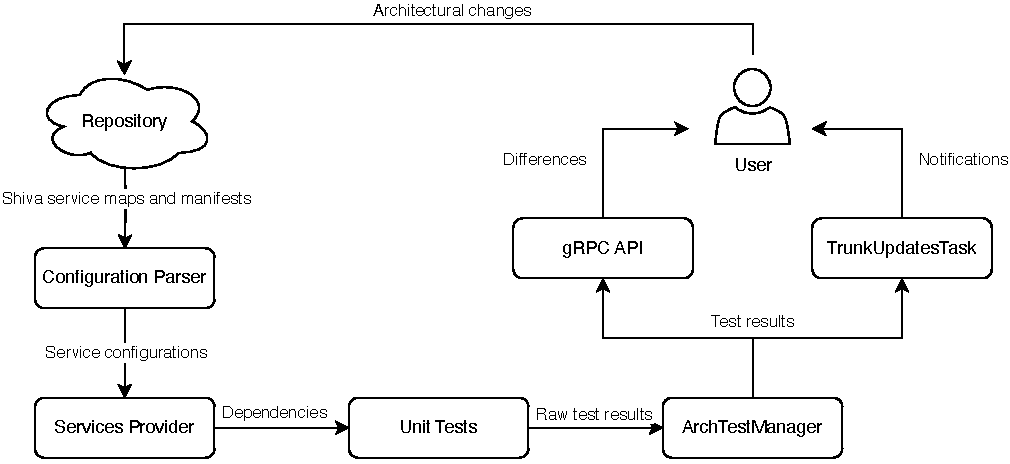
\includegraphics[scale=0.9]{images/archtest-components.drawio.pdf}
    \caption{\label{archtest-components} Ключевые компоненты и их взаимодействие.}
\end{figure}

Основные компоненты приложения, а также их взаимодействие между собой и с пользователем представлено на рисунке \ref{archtest-components}. Таким образом, приложение состоит из нескольких модулей:

\begin{itemize}
    \item \textbf{Модуль загрузки и парсинга конфигураций}. Отвечает за получение данных об архитектуре анализируемой системы.
    \item \textbf{Архитектурные правила}. Могут быть заданы двумя способами: в виде unit-тестов на языке Scala или декларативно в формате YAML.
    \item \textbf{Модуль выполнения тестов}. Управляет процессом запуска архитектурных проверок и выставляет программное API для получения агрегированных результатов прогона тестов.
    \item \textbf{gRPC API} \cite{grpc-fw}. Предоставляет удобные методы для интеграции инструмента с CI/CD и автоматической проверки изменений в пулл-реквестах.
    \item \textbf{TrunkUpdatesTask}. Отслеживает изменения в основной ветке разработки (trunk \cite{trunk-based-dev}) и отправляет уведомления в Telegram при обнаружении новых архитектурных проблем.
\end{itemize}

В следующих разделах будет подробно рассмотрен каждый из перечисленных компонентов.

\subsection{Загрузка и парсинг конфигураций}

Источником данных для тестов служат конфигурационные файлы системы развертывания Shiva: карты сервисов и манифесты деплоя. Инструмент умеет получать эти файлы либо из системы контроля версий Arcadia \cite{arcadia} для указанной ревизии (коммита или ветки), либо из локальной файловой системы. Это позволяет анализировать как любой заданный срез архитектуры в прошлом, так и текущее локальное состояние. Загруженные YAML-файлы проходят через стадию парсинга и преобразуются во внутреннюю модель системы. Эта модель представляет собой граф, узлами которого являются сущности типа \verb|Service|, а рёбрами — зависимости между ними. Каждый объект \verb|Service| содержит информацию об имени сервиса, его типе, предоставляемых интерфейсах и зависимостях: как явных, указанных в \verb|depends_on|, так и неявных, содержащихся в переменных окружения из конфигурации. Помимо этих полей в \verb|Service| содержится и другая метаинформация о сервисе, которую предоставляет Shiva.

\subsection{Написание unit-тестов}\label{unit-tests-design}

Основным и наиболее гибким способом описания архитектурных правил является создание unit-тестов на языке Scala с использованием фреймворка ScalaTest \cite{scalatest-fw}. Для этого разработчикам предоставляется специальный трейт \verb|ArchTest|, который необходимо унаследовать в классе с тестами. Этот трейт обеспечивает доступ к загруженной и обработанной модели архитектуры, а также предоставляет вспомогательные методы для написания проверок. Как уже упоминалось, при локальном запуске тестов будет использована текущая локальная конфигурация сервисов Shiva.

Вместо построения явного графа зависимостей, здесь используется несколько другой подход: \verb|ArchTest| предоставляет список всех сервисов \verb|services: Seq[Service]|, внутри каждого из которых содержится вся информация о его зависимостях. Чтобы проверить наличие зависимости между сервисами \verb|A| и \verb|B|, нужно вызвать метод \verb|hasDependencyOn| у \verb|A|. Метод просканирует секцию \verb|depends_on| и все переменные окружения сервиса \verb|A| на упоминание сервиса \verb|B|. Если оно будет найдено, то метод возвращает \verb|true|. Более формально это отражено в алгоритме \ref{has-dependency-on}.

\begin{algorithm}[hbt!]
\caption{Проверка зависимости от другого сервиса}\label{has-dependency-on}

\SetKwProg{hasDependencyOn}{hasDependencyOn}{}{}
\hasDependencyOn{$(this, other)$}{
\KwData{$this$ — текущий сервис со своими зависимостями}
\KwData{$other$ — другой сервис для проверки}

$inDependsOn \gets \text{false}$\;
\ForEach{$dependency \in this.dependsOn$}{
    \If{$\text{matches}(other, dependency)$}{
        $inDependsOn \gets \text{true}$\;
        \textbf{break}\;
    }
}

$inConfig \gets \text{false}$\;
\ForEach{$envVariable \in this.config.envVariables$}{
    \If{$\text{matches}(other, envVariable)$}{
        $inConfig \gets \text{true}$\;
        \textbf{break}\;
    }
}

\Return $inDependsOn \lor inConfig$\;
}
\end{algorithm}

Алгоритм использует функцию \verb|matches|, чтобы проверить совпадение сервиса \verb|other| с очередным сервисом из \verb|depends_on| или с очередной переменной окружения \verb|envVariable|. Подробнее про внутреннее устройство этой функции будет написано в одном из следующих разделов, а пока что можно воспринимать её работу <<естественно>>: сервисы могут совпасть по имени, по URL и так далее.

Помимо основного \verb|hasDependencyOn|, библиотека предоставляет другие полезные функции для разных сценариев использования:

\begin{itemize}
    \item \verb|hasDependencyInServiceMap|: Проверяет только явные зависимости из \verb|depends_on|.
    \item \verb|hasDependencyInConfig|: Проверяет только зависимости, выведенные из переменных окружения (например, URL другого сервиса или строки подключения к БД).
    \item \verb|hasDependencyOn(other: ServicePattern)|: Работает аналогично основному методу, но принимает не существующий в системе \verb|Service|, а описанный пользователем \verb|ServicePattern|. Паттерн позволяет гибко задавать критерии поиска целевого сервиса (по имени, типу, хосту, IP-адресу и так далее).
\end{itemize}

Для иллюстрации рассмотрим простой пример теста, который проверяет, что сервис \verb|payment-service| не должен напрямую зависеть от базы данных пользователей \verb|user-db| (допустим, что такие компоненты есть в нашей системе).

\begin{code}{scala}
"payment-service" should "not access user-db" in {
  val paymentService = Services.service("payment-service")
  val userDb = Services.mysql("user-db")

  paymentService.hasDependencyOn(userDb) shouldBe false
}
\end{code}

\verb|Services.service("payment-service")| является удобным способом получить экземпляр \verb|Service| для сервиса с именем "payment-service". Для базы данных \verb|user-db| используется аналогичный метод \verb|Services.mysql|.

Другой пример: проверка, что только \verb|orders-proxy| может зависеть от внешней системы \verb|orders.com|.

\begin{code}{scala}
"orders.com" should "only be accessed by orders-proxy" in {
  val ordersProxy = Services.service("orders-proxy")
  val ordersCom = ServicePattern.withHost("orders.com")

  val ordersComDependents = services.filter { service =>
    service.hasDependencyOn(ordersCom)
  }

  ordersComDependents shouldBe Seq(ordersProxy)
}
\end{code}

Здесь мы итерируемся по всем сервисам и проверяем условие, что только прокси имееет прямую зависимость на внешнюю систему.

\subsection{Задание проверок в YAML-конфиге}

Для простых и типовых архитектурных правил инструмент позволяет описывать их в декларативном стиле с помощью YAML-файлов \cite{yaml-spec}. Это может быть удобно для для быстрого добавления стандартных проверок без написания Scala-кода.

Каждый YAML-файл может содержать список правил. Структура правила определяется следующими полями:
\begin{itemize}
    \item \verb|rule|: Человекочитаемое описание правила.
    \item \verb|service|: Определяет сервис или группу сервисов, к которым применяется правило. Содержит обязательное поле \verb|name|, значение которого интерпретируется как регулярное выражение для полного имени сервиса (например, \verb|mysql/user-db| или \verb|payment-service|). Структура задумывалась расширяемой, чтобы в дальнейшем можно было задавать сервис не только по имени, а, например, по владельцу или другой метаинформации.
    \item \verb|dependencies| (опционально): Определяет ограничения на исходящие зависимости проверяемого сервиса. Может содержать либо \verb|whitelist| (список разрешенных сервисов-зависимостей), либо \verb|blacklist| (список запрещенных сервисов-зависимостей). Элементы в \verb|whitelist| и \verb|blacklist| являются <<сервисами>>, то есть могут быть также заданы по имени с помощью регулярного выражения.
    \item \verb|dependents| (опционально): Определяет ограничения на входящие зависимости (сервисы, которые зависят от проверяемого сервиса). Структура аналогична \verb|dependencies|.
\end{itemize}

Важно, что в рамках одного блока (\verb|dependencies| или \verb|dependents|) нельзя одновременно использовать \verb|whitelist| и \verb|blacklist|, так как это не имеет смысла.

Для иллюстрации возможностей правил в YAML, перепишем unit-тест про \verb|payment-service| из предыдущего раздела декларативно.

\begin{nocode}
- rule: "payment-service should not access user-db"
  service:
    name: mysql/user-db
  dependents:
    blacklist:
      - name: payment-service
\end{nocode}

Другой пример: сервисы catalog-api и catalog-tasks не должны ни от кого зависеть.

\begin{nocode}
- rule: "catalog should not depend on other services"
  service:
    name: catalog-(api|tasks)
  dependencies:
    whitelist: []
\end{nocode}

Разбор и выполнение таких YAML-правил осуществляется специальным ScalaTest-тестом \verb|YamlSpec|. Он находит все \verb|*.yml| файлы в заданной директории, парсит их и для каждого правила из файла динамически генерирует соответствующие проверки во время выполнения тестов.

\subsection{Запуск тестов в рантайме}

Библиотека для написания архитектурных тестов разработана таким образом, чтобы их можно было запускать не только локально из IDE, но и программно, например, по запросу или периодически. Эту функциональность обеспечивает \verb|ArchTestManager|. Когда \verb|ArchTestManager| получает запрос на запуск тестов для определённой ревизии (коммита или имени ветки), ему необходимо каким-то образом передать в тесты нужную версию инфраструктурных схем. Для этого он устанавливает системное свойство JVM \verb|archtest.run_mode|. Значением этого свойства является JSON-строка, представляющая объект \verb|RunMode|, например,

\begin{zerocode}{json}
{
    "mode": "Branch",
    "revision": "my-feature-branch",
    "arc_config": {
        "token": "<ARC_TOKEN>",
        "path": "/opt/homebrew/bin/arc"
    }
}
\end{zerocode}

Использование \verb|System.setProperty| для передачи параметров запуска является ключевым моментом. Стандартный механизм \verb|ConfigMap| из ScalaTest здесь не подходит, поскольку он становится доступен уже после обнаружения и инициализации тестовых классов. В нашем же случае, конфигурация (режим запуска, ревизия) нужна на самом раннем этапе – до того, как ScalaTest начнет исполнять тесты, и даже до того как он полностью определит их список. Это связано с тем, что сама структура архитектуры (и, как следствие, набор сервисов, для которых могут генерироваться тесты) зависит от выбранной ревизии.

После установки системного свойства, \verb|ArchTestManager| запускает стандартный \verb|scalatest.Runner|. Он обнаруживает все скомпилированные тестовые классы, и при инстанцировании каждого такого класса, благодаря подмешанному трейту \verb|ArchTest|, происходит следующее:

\begin{enumerate}
    \item Читается системное свойство \verb|archtest.run_mode|.
    \item На основе этого свойства выбирается и конфигурируется соответствующий провайдер данных (например, \verb|ServicesProviderArcadia| для режима \verb|Branch|).
    \item Выбранный провайдер загружает конфигурационные файлы Shiva для заданной ревизии (из Arcadia или локально).
    \item Загруженные файлы парсятся, и строится полная внутренняя модель системы в виде последовательности объектов \verb|Seq[Service]|.
    \item Эта модель становится доступной внутри тестового класса через поле \verb|lazy val services: Seq[Service]|, и уже на ее основе выполняются проверки.
\end{enumerate}

Результаты выполнения тестов (успех/неудача, сообщения об ошибках и т.д.) собираются с помощью кастомной реализации \verb|scalatest.Reporter|. Он подписывается на события \verb|TestSucceeded| и \verb|TestFailed|, которые генерирует ScalaTest во время выполнения тестов, и собирает информацию о результатах прогона. В итоге они возвращаются в виде структурированных объектов \verb|RunTestResult| в вызывающий код.

\subsection{Валидация изменений в пулл реквесте}

Одна из основных задач инструмента — предотвращение попадания нежелательных архитектурных изменений в основную ветку разработки (trunk). Для этого инструмент предоставляет возможность сравнить результаты архитектурных тестов между текущей веткой разработки (например, веткой пулл-реквеста) и её точкой расхождения с trunk, так называемой merge-base. Эта логика реализована в \verb|ArchTestManager| и доступна через gRPC-метод \verb|compareTestsWithTrunk|.

При вызове этого метода с указанием имени проверяемой ветки, gRPC-сервис определяет merge-base и дважды запускает архитектурные тесты: для указанной ветки и для merge-base. После этого результаты двух запусков сравниваются, и выделяются различия: новые упавшие тесты (потенциальные проблемы), исправленные тесты (улучшения), а также добавленные или удаленные тесты. Эта информация возвращается через gRPC и может быть использована CI/CD системой для автоматического комментирования пулл-реквеста, информируя разработчиков и ревьюеров о влиянии предлагаемых изменений на архитектуру.

На данный момент, непосредственная интеграция с интерфейсом систем управления версиями (в случая Яндекса — это Arcanum) для публикации комментариев в пулл-реквестах не реализована, так как было принято решение сначала провести апробацию инструмента и оценку его эффективности в более узком кругу разработчиков. Однако весь необходимый функционал на стороне бэкенда для такой интеграции уже существует и запущен в облаке.

\subsection{Уведомления в Telegram}

В качестве основного способа обратной связи на текущем этапе и для поэтапного внедрения инструмента была выбрана система уведомлений об архитектурных изменениях в основной ветке (trunk) через Telegram. Это решение является временной альтернативой полноценной интеграции проверок в процесс код-ревью, позволяя избежать немедленной раскатки новой функциональности на всех разработчиков компании (которые неизбежно столкнулись бы с инструментом при работе с пулл-реквестами). Такой подход даёт возможность узкому кругу заинтересованных лиц апробировать инструмент, собрать обратную связь и оценить его пользу в реальных условиях без широкого анонсирования. Реализацию этого непрерывного мониторинга обеспечивает фоновая задача \verb|TrunkUpdatesTask|. Важно отметить, что даже после полного запуска валидации в пулл-реквестах, \verb|TrunkUpdatesTask| сохранит свою актуальность: она будет служить дополнительным уровнем контроля для архитекторов, информируя их о случаях, когда архитектурные нарушения все же могли быть пропущены или сознательно внесены в основную ветку разработки.

\verb|TrunkUpdatesTask| с настраиваемой периодичностью запрашивает историю коммитов в репозиторий с инфраструктурными схемами Shiva. Для каждой пары последовательных коммитов (старый и новый) запускается сравнение результатов архитектурных тестов. Если обнаруживаются различия (например, тест, который проходил в старом коммите, начал падать в новом, или наоборот), формируется соответствующее уведомление в Telegram.

Ключевую роль в системе уведомлений играет механизм тегирования результатов тестов и конфигурация подписок.
Система уведомлений может понимать контекст упавшего или исправленного теста и отправлять сообщение только тем, кому данный тест может быть интересен. Для этого все тесты снабжаются тегами с помощью метода \verb|report|. Предусмотрено несколько способов вызова:
\begin{itemize}
    \item \verb|report(service: Service*)|: Автоматически добавляет стандартный набор тегов для указанных сервисов: их полное имя, владельцев и некоторые другие поля. Например, \verb|report(myService)| добавит тег \verb|"fqn": "my-service"|, \verb|"owner": "..."| и так далее. Более того, для удобства написания тестов сделано так, что обращение к функции \verb|Services.service| само по себе вызывает \verb|report| на переданном сервисе.
    \item \verb|report(key: String, value: String)|: Добавляет пользовательский тег, например, \verb|report("tag", "critical")|.
\end{itemize}

Технически, метод \verb|report| вызывает \verb|note| из ScalaTest, передавая строку с тегами в специальном формате. Уже упомянутый ранее кастомный \verb|scalatest.Reporter| перехватывает события \verb|NoteProvided| и извлекает теги, прикрепляя их к результату соответствующего теста (\verb|RunTestResult|).

Сформированные уведомления и ассоциированные с ними теги передаются в \verb|TelegramNotifier|. Последний, на основе конфигурации подписок, определяет, каким пользователям или в какие чаты следует отправить сообщение. Конфигурация подписок загружается в рантайме из системы управления фича-флагами и представляет собой YAML-структуру следующего вида:

\begin{itemize}
    \item \verb|name|: Человекочитаемое описание подписки.
    \item \verb|enabled|: Включена ли данная подписка или нет.
    \item \verb|chat_ids|: Список числовых ID чатов Telegram, куда нужно отправлять уведомления по данной подписке.
    \item \verb|conditions|: Список условий для срабатывания подписки. Сообщение будет отправлено, если результат теста удовлетворяет всем условиям из этого списка (логическое "И"). Каждое условие — это пара, где ключ — это имя тега (например, \verb|fqn|, \verb|owner|, \verb|tag| и т.д.), а значение — список допустимых строковых значений. Для того чтобы условие по ключу считалось выполненным, тег с таким ключом у результата теста должен иметь хотя бы одно из значений, перечисленных в списке (логическое "ИЛИ"). Например, условие \verb|fqn: ["service-a", "service-b"]| сработает, если имя сервиса, связанного с тестом, равняется \verb|service-a| или \verb|service-b|.
\end{itemize}

Ниже приведен пример с двумя подписками на уведомления.

\begin{nocode}
subscriptions:
  - name: "Critical issues for Team A"
    enabled: true
    chat_ids:
      - 123456789
      - 987654321
    conditions:
      - tag: ["critical"] 
      - owner: ["team-a"]
  - name: "All payment service issues"
    enabled: true
    chat_ids:
      - 112233445 
    conditions:
      - fqn: ["payment-api", "payment-tasks"]
\end{nocode}

Пример уведомления в Telegram показан на рисунке \ref{telegram-notification-example}.

\section{Внутреннее устройство библиотеки написания тестов}

В данном разделе будет рассмотрено внутреннее устройство библиотеки для написания архитектурных тестов. Библиотека предоставляет разработчикам высокоуровневое API, абстрагируя их от деталей парсинга конфигурационных файлов и представления архитектуры. Центральное место в этом API занимают методы объекта \verb|Service|, позволяющие проверять наличие зависимостей. Далее будут подробно описаны основные концепции, компоненты и алгоритмы, лежащие в основе этого механизма. 

\subsection{Основные подходы к написанию тестов}

Как было показано в разделе \ref{unit-tests-design}, написание архитектурных тестов сводится к вызову методов на экземплярах класса \verb|Service|
\begin{itemize}
    \item \verb|hasDependencyOn(service: Service): Boolean|
    \item \verb|hasDependencyOn(service: ServicePattern): Boolean|
    \item и так далее
\end{itemize}

\begin{code}{scala}
val serviceA = Services.service("service-a")
val serviceB = Services.service("service-b")
serviceA.hasDependencyOn(serviceB) shouldBe true

val ordersCom = ServicePattern.withHost("orders.com")
serviceA.hasDependencyOn(ordersCom) shouldBe false
\end{code}

Эти методы инкапсулируют логику поиска зависимостей как в явно декларированной секции \verb|depends_on| в карте сервиса, так и в переменных окружения, указанных в манифесте деплоя. Внутренний механизм, обеспечивающий эту функциональность, основан на гибкой системе сопоставления (matching), реализованной с помощью трейта \verb|Matchable|.

\subsection{Механизм сопоставления зависимостей}

\verb|Matchable[A, B]| определяет единственный метод \verb|matches(a, b)|, который возвращает \verb|true|, если объект \verb|a| типа \verb|A| <<соответствует>> объекту \verb|b| типа \verb|B| по некоторым критериям.

\begin{code}{scala}
trait Matchable[A, B] {
  def matches(a: A, b: B): Boolean
}
\end{code}

Такой подход позволяет абстрагироваться от конкретных способов сравнения сервисов или их атрибутов, предоставляя возможность легко подменять и комбинировать различные стратегии сопоставления.

\subsubsection{Поиск зависимости в секции depends\_on}

Для проверки, содержится ли сервис \verb|other| в списке явных зависимостей \verb|depend_on|, используется метод \verb|hasDependencyInServiceMap|. Он пробегается по списку зависимостей сервиса и пытается найти среди них совпадение с переданным \verb|other|.

Например, сервис, объявленный в коде как

\begin{codenl}{scala}
val serviceA = ServicePattern
  .withName("serviceA")
  .withInterfaceName("grpc-api")
\end{codenl}

должен <<соответствовать>> следующей записи в карте сервисов:

\begin{nocode}
depends_on:
  - service: service-a
    interface_name: grpc-api
\end{nocode}

При парсинге YAML-файла, эта запись преобразуется в экземпляр \verb|ServicePattern|. Таким образом, задача сводится к сопоставлению двух \verb|ServicePattern|: \verb|other| и полученного из списка \verb|dependsOn|. А это равносильно написанию \verb|Matchable[ServicePattern, ServicePattern]|.

Библиотека предоставляет экземпляр такого \verb|Matchable| по умолчанию. Он сравнивает сервисы по имени, типу и интерфейсам. Тем не менее, при необходимости пользователь может определить и передать в функцию свой собственный экземпляр \verb|Matchable|.

\subsubsection{Поиск зависимости в конфигурационных файлах}

Аналогичный подход используется для поиска зависимостей, косвенно определённых через переменные окружения в конфигурационных файлах сервиса.

Например, сервис:

\begin{codenl}{scala}
val serviceA = ServicePattern
  .withName("serviceB")
  .withInterfaceName("http-api")
\end{codenl}

может быть упомянут в конфигурации другого сервиса через различные переменные окружения: 

\begin{nocode}
SERVICE_B_HOST: ${host:service-b:http-api}
SERVICE_B_URL: service-b-http-api.yandex.net
\end{nocode}

Для обнаружения подобных неявных зависимостей достаточно пробежаться по списку переменных окружения сервиса с экземпляром \verb|Matchable| для \verb|ServicePattern| и \verb|EnvVariable|, где \verb|EnvVariable| — это простая структура, представляющая пару ключ-значение переменной окружения.

Аналогично поиску в depends\_on, библиотека предоставляет экземпляр нужного \verb|Matchable| по умолчанию. Он способен распознавать различные форматы указания зависимостей: URL, внутренние шаблоны Shiva, строки подключения к базам данных, указания на топики Kafka и многое другое.

\subsubsection{Гибкость и композируемость Matchable}

Ключевое преимущество трейта \verb|Matchable| заключается в его гибкости и возможности композиции. Поскольку типы \verb|A| и \verb|B| не зафиксированы, можно создавать экземпляры \verb|Matchable| для совершенно разных пар типов и комбинировать их для построения сложной логики сопоставления.

Существует два подхода к созданию экземпляров \verb|Matchable|. Более прямолинейный подход заключается в том, что можно определить экземпляр \verb|Matchable| как обычную функцию. Например, для сопоставления двух сервисов по их IP-адресам, можно написать следующее:

\begin{code}{scala}
val matchServicesByIp: Matchable1[ServicePattern] =
  (a: ServicePattern, b: ServicePattern) =>
    (a.ip, b.ip) match {
      case (Some(ipA), Some(ipB)) => ipA == ipB
      case _ => false
    }
\end{code}

Здесь и далее тип \verb|type Matchable1[A] = Matchable[A, A]| определен для удобства. 

С прямолинейным подходом получилось не сложнее, чем определить обычную функцию. Правда, переиспользовать такой код вряд ли получится. 

Второй подход отличается от первого и активно использует композицию. Библиотека предоставляет набор функций-конструкторов и комбинаторов, позволяющих собирать сложные \verb|Matchable| из более простых «строительных блоков».

\begin{itemize}
    \item \verb|byEquals[A]|: Создает \verb|Matchable1[A]|, который проверяет равенство переданных значений.    

\begin{codenl}{scala}
def byEquals[A]: Matchable1[A] =
  (a1: A, a2: A) => a1 == a2
\end{codenl}

    \item \verb|lift[A, B, C, D]|: <<Поднимает>> \verb|Matchable[A, B]| до \verb|Matchable[C, D]|, если есть способы преобразовать \verb|C| в \verb|A| и \verb|D| в \verb|B|.

\begin{codenl}{scala}
def lift[A, B, C, D](
    m: Matchable[A, B]
  )(ca: C => A, 
    db: D => B): Matchable[C, D] = 
  m.matches(ca(c), db(d))
\end{codenl}

    \item \verb|lift1[A, C]|: Сокращенная версия \verb|lift[A, B, C, D]| для случая, когда \verb|A == B| и \verb|C == D|.

\begin{codenl}{scala}
def lift1[A, C](
    m: Matchable1[A]
  )(ca: C => A): Matchable1[C] =
  lift[A, A, C, C](m)(ca, ca)
\end{codenl}

    \item \verb|options[A, B]|: Преобразует \verb|Matchable[A, B]| в версию с \verb|Option|. Сопоставление происходит, только если оба \verb|Option| содержат значения.

\begin{codenl}{scala}
def options[A, B](
    m: Matchable[A, B]
  ): Matchable[Option[A], Option[B]] = {
  case (Some(a), Some(b)) => m.matches(a, b)
  case _ => false
}
\end{codenl}

\end{itemize}

Используя эти конструкторы, пример \verb|matchServicesByIp| можно переписать по-другому.

\begin{code}{scala}
val matchStrings: Matchable1[String] = 
  byEquals[String]

val matchIps: Matchable1[Ip] =
  matchStrings.lift1[Ip](_.value)

val matchServicesByIp: Matchable1[ServicePattern] =
  matchIps.options.lift1[ServicePattern](_.ip)
\end{code}

Для улучшения читаемости кода, объявления стандартных функций вроде \verb|lift1| или \verb|options| продублированы в implicit-классах, что позволяет использовать их через точечную нотацию: \verb|matchIps.options.lift1(_.ip)|. Такой подход, хоть и кажется более многословным для простого случая, обеспечивает высокую степень переиспользования промежуточных \verb|Matchable|.

Библиотека также определяет функции \verb|or| и \verb|and| для комбинации нескольких \verb|Matchable|.

\begin{codenl}{scala}
def or[A, B](inners: Matchable[A, B]*): Matchable[A, B] =
  (a: A, b: B) => inners.exists(_.matches(a, b))

def and[A, B](inners: Matchable[A, B]*): Matchable[A, B] =
  (a: A, b: B) => inners.forall(_.matches(a, b))
\end{codenl}

Это позволяет выражать сложные условия сопоставления очень компактно. Например, стандартный \verb|Matchable1[ServicePattern]|, который используется по умолчанию, определен в библиотеке следующим образом.

\begin{code}{scala}
val byIp: Matchable1[ServicePattern] = 
  matchIps.options.lift1[ServicePattern](_.ip)

// byHost, byFqn, byInterfaces аналогично byIps

val matchServices: Matchable1[ServicePattern] =
  byIp or byHost or (byFqn and byInterfaces)
\end{code}

То есть сервисы считаются совпадающими, если у них совпадает IP-адрес, или хост, или одновременно полное имя сервиса и его интерфейсы.

\subsection{Прямой доступ к конфигурационным данным}

Хотя использование \verb|Matchable| является предпочтительным и наиболее гибким способом определения критериев сопоставления, иногда может потребоваться прямой доступ к сырым данным конфигурации. Библиотека оставляет такую возможность, предоставляя доступ к списку всех переменных окружения сервиса через поле \verb|config.all: Seq[EnvVariable]|.

Это может быть полезно для написания специфических проверок, которые сложно или нецелесообразно выражать через \verb|Matchable|. Таким образом разработчик тестов не ограничен предопределенными механизмами \verb|Matchable| и может реализовывать любую необходимую логику.

Рассмотрим пример теста, который проверяет, что у сервиса \verb|api-gateway| нет внешних зависимостей.

\begin{code}{scala}
"api-gateway" should "not have external dependencies" in {
  val apiGateway = Services.service("api-gateway")
  val envVariables = apiGateway.config.all
  envVariables.count(isExternalService) shouldBe 0
}
\end{code}

Тест использует функцию \verb|isExternalService|, которая по значению переменной окружения определяет, внешняя это зависимость или нет. Конкретная реализация функции опущена для краткости.

\subsection{Оптимизации для повышения производительности}

При анализе больших архитектур с сотнями сервисов и тысячами конфигурационных параметров производительность проверок становится важным фактором. В библиотеке реализовано несколько оптимизаций для ускорения процесса сопоставления зависимостей.

\subsubsection{Кеширование результатов сопоставления}

Тесты могут быть написаны таким образом, что одна и та же пара сервисов будет проверяться на наличие зависимости между ними несколько раз. В таком случае логично кешировать результаты сопоставления внутри экземпляра класса \verb|Service|, чтобы не вычислять их каждый раз заново.

При вызове методов типа \verb|hasDependencyOn| результат сначала ищется в соответствующем кеше. Если для данного аргумента \verb|ServicePattern| результат уже был вычислен ранее, он возвращается немедленно. В противном случае, выполняется честное сопоставление, и результат сохраняется в кеш для последующих вызовов. 
% Более формально это продемонстрировано в алгоритме \ref{has-dependency-on-cached}.

% \begin{algorithm}[hbt!]
% \caption{Проверка зависимости от другого сервиса c кешированием}\label{has-dependency-on-cached}

% \SetKwProg{hasDependencyOn}{hasDependencyOn}{}{}
% \hasDependencyOn{$(this, other, cache)$}{
% \KwData{$this$ — текущий сервис со своими зависимостями}
% \KwData{$other$ — другой сервис для проверки}
% \KwData{$cache$ — кеш с результатами предыдещих вызовов}

% \If{$other \notin cache$}{
%     $cache[other] \gets hasDependencyOn(this, other)$\;
% }

% \Return $cache[other]$\; 
% }
% \end{algorithm}

Оптимизация валидна, так как граф зависимостей не может поменяться во время выполнения тестов. При этом она срабатывает только при передаче стандартных экземпляров \verb|Matchable|, так как от конкретной реализации трейта зависит результат выполнения функции.

Кеширование обладает небольшими накладными расходами, но зато значительно сокращает количество повторных вычислений, особенно в сценариях с большим количеством тестов.

\subsubsection{Эвристики для ускорения сопоставления}

Наиболее дорогостоящая операция при выполнении тестов — это поиск зависимостей в конфигурационных файлах, так как он требует итерации по всем переменным окружения и применения к ним потенциально сложных правил \verb|Matchable|. Для ускорения этого и других процессов в библиотеке реализован ряд эвристик и подходов.

Во-первых, это эвристика \verb|skimConfig|, которая применяется перед полным сканированием конфигурации на наличие зависимости от сервиса \verb|other|. Если \verb|other| определён только по своему имени (что верно для большинства сервисов), метод быстро проверяет, содержится ли строка с именем этого сервиса в конкатенированном значении всех переменных окружения. Если имя не найдено, то детальное сопоставление с помощью \verb|Matchable| можно пропустить, так как зависимость по имени точно отсутствует. Эвристика не влияет на корректность результатов, так как используется только тогда, когда ее вывод является гарантированно верным. Эффективность данной схемы обусловлена тем фактом, что граф зависимостей скорее всего будет разреженным, то есть функция \verb|hasDependencyOn| гораздо чаще будет возвращать \verb|false|, чем \verb|true|. При этом поиск подстроки в строке выполняется гораздо быстрее честного сопоставления. В итоге, общий выигрыш в производительности достигается за счет того, что быстрое исключение большинства \verb|false|-случаев легко компенсирует незначительные накладные расходы на выполнение этой предварительной проверки в более редких \verb|true|-случаях.

Во-вторых, для выполнения массовых операций над всеми сервисами системы, таких как фильтрация или поиск, библиотека предоставляет параллельную коллекцию \verb|servicesPar: ParSeq[Service]|, использование которой в тестах позволяет задействовать многопоточность. Стоит отметить, что не всегда замена \verb|services| на \verb|servicesPar| даёт выигрыш, однако грамотное её использование также повышает производительность.

В-третьих, повсеместно применяется стратегия <<дешевых предварительных проверок>> перед выполнением дорогих операций. Например, известно, что любой внутренний шаблон Shiva для задания хоста сервиса начинается со знака \verb|'$'|. Поэтому перед применением сложного регулярного выражения, которое бы распарсило шаблон, сначала выполняется простая проверка, что первый символ строки является \verb|'$'|. Если нет, то применение регулярного выражения не производится, что немного ускоряет выполнение.

Эти основные оптимизации, вместе с другими, менее значительными улучшениями, позволили ускорить выполнение набора архитектурных тестов более чем в полтора раза. Если также учитывать выигрыш и от кеширования результатов сопоставления, то общая скорость выполнения тестов увеличилась почти в 2.5 раза по сравнению с вариантом без оптимизаций. Важно подчеркнуть, что точное измерение производительности не входило в задачи данной работы, поэтому приведённые значения являются оценочными и могут отличаться для разных наборов тестов и конфигураций оборудования. Тем не менее, можно утверждать, что после оптимизаций процесс анализа архитектуры заметно ускорился.

\section{Применение на реальных микросервисных системах}

Для оценки практической применимости и эффективности разработанного инструмента был проведен его запуск на нескольких реальных микросервисных системах, разрабатываемых в Яндекс.Вертикалях. В данном разделе будут представлены итоги этого эксперимента, включая примеры реализованных архитектурных тестов и анализ полученных результатов. 

\subsection{Описание целевых систем}

Запуск инструмента проводился на четырех различных микросервисных системах, условно обозначенных как А, B, C и D. Все четыре системы представляют собой сложные, распределенные приложения внушительного масштаба:

\begin{itemize}
    \item \textbf{Система А}: включает в себя около 550 отдельных компонентов (микросервисы, базы данных, очереди сообщений и т.д.). 
    \item \textbf{Система B}: состоит из 300 компонентов. 
    \item \textbf{Система C}: насчитывает 400 компонентов. 
    \item \textbf{Система D}: включает 150 компонентов. 
\end{itemize}

Названия систем и точное число компонентов не приводятся в целях сохранения внутренней информации компании. Во всех последующих примерах названия конкретных сервисов также изменены по тем же соображениям.

Для лучшего понимания масштаба исследуемых систем отметим, что, по открытым данным, в 2023 году известный сервис Яндекс.Еда функционировал на основе около 180 различных микросервисов, то есть имел сопоставимые системам A-D размеры \cite{yandex-eda-ms-count}.

\subsection{Обнаруженные архитектурные антипаттерны}

В ходе эксперимента был реализован набор тестов и правил, нацеленных на выявление как общеизвестных архитектурных антипаттернов, так и нарушений специфичных для конкретных систем.

\subsubsection{Shared Database}

Антипаттерн Shared Database (Общая база данных) возникает, когда несколько независимых сервисов совместно используют одну и ту же базу данных. Разработанный тест проверяет, что каждая база данных используется не более чем одним сервисом или одной логической группой сервисов. Под логической группой подразумевается ситуация, когда один сервис физически разделён на несколько компонентов, например, когда API сервиса и его асинхронные задачи реализованы как разные развертываемые единицы. 

\begin{code}{scala}
"Each database" should {
  services
    .filter(_.isDatabase)
    .foreach { database =>
      s"be used by only one service: ${database.fqn}" in {
        val dependents = services
          .filter(_.hasDependencyOn(database))

        fromOneServiceGroup(dependents) shouldBe true
      }
    }
}
\end{code}

Вспомогательная функция \verb|fromOneServiceGroup| определяет принадлежность сервисов-потребителей к одной логической группе, например, по общему префиксу имени или другим метаданным. Конкретная реализация данной функции для краткости опущена.

Данный тест обнаружил 4 общие базы данных в системе A и по одной в системах B и D.

\subsubsection{Lava Flow}

Антипаттерн Lava Flow (Поток лавы) описывает накопление в системе устаревших и неиспользуемых компонентов. Это могут быть базы данных, сервисы или топики Kafka, на которые ни один другой компонент системы уже не зависит. 

Тест для поиска неиспользуемых баз данных:

\begin{code}{scala}
"Each database" should {
  services
    .filter(_.isDatabase)
    .foreach { database =>
      s"be used: ${database.fqn}" in {
        val dependents = services
          .filter(_.hasDependencyOn(database))

        dependents should not be empty
      }
    }
}
\end{code}

Тест для поиска неиспользуемых API-сервисов выглядит аналогично. Отметим, что проверять таким образом сервисы, которые не выставляют API, не имеет смысла, так как на них в принципе нельзя зависеть в рамках построенного графа.

\begin{code}{scala}
"Each API service" should {
  services
    .filter(_.isService)
    .filter(_.provides.nonEmpty) // provides some API
    .foreach { service =>
      s"be used: ${service.fqn}" in {
        val dependents = services
          .filter(_.hasDependencyOn(service))

        dependents should not be empty
      }
    }
}
\end{code}

С топиками Kafka ситуация несколько сложнее: тест должен проверить, что у каждого топика есть хотя бы один продюсер и хотя бы один консьюмер. Также необходимо учесть, что одна очередь сообщений (представленная как один компонент в графе зависимостей) может предоставлять несколько топиков, каждый из которых тест должен обработать отдельно. 

\begin{code}{scala}
"Each kafka topic" should {
  val topics = Services.Kafka.provides.map { topic =>
    // kafka with only one topic
    Services.Kafka.copy(provides = Seq(topic))
  }

  topics.foreach { topic =>
    val topicName = topic.provides.head.name.value

    s"have producer and consumer: $topicName" in {
      val dependents = services
        .filter(_.hasDependencyOn(topic))
      val producers = dependents
        .filter(_.isKafkaProducerFor(topicName))
      val consumers = dependents
        .filter(_.isKafkaConsumerFor(topicName))

      producers should not be empty
      consumers should not be empty
    }
  }
}
\end{code}

Вышеописанные тесты помогли обнаружить 29 неиспользуемых сервисов, 5 неиспользуемых баз данных и 28 Kafka-топиков без продюсера или консьюмера: 17 сервисов, 2 базы данных и 9 топиков в системе А; 4 сервиса и 6 топиков в системе B; 6 сервисов, 2 базы данных и 4 топика в системе C; 2 сервиса, 1 база данных и 9 топиков в системе D. 

Важно отметить, что не все из обнаруженных <<неиспользуемых>> компонентов действительно являются таковыми. Некоторые сервисы могут быть предназначены для внешних интеграций, и поэтому внутренние зависимости на них отсутствуют. Также несколько сервисов на момент запуска тестов находились в фазе активной разработки, поэтому формальные зависимости на них еще не были установлены, что, конечно, не является архитектурной проблемой. Более подробный анализ количества ложноположительных срабатываний будет сделан в конце данного раздела.

\subsubsection{Cyclic Dependency}

Антипаттерн Cyclic Dependency (Циклическая зависимость \cite{cyclic-dep-ap}) между компонентами усложняет развертывание, тестирование и общее понимание системы. Тест ниже находит двусторонние циклические зависимости (циклы длины 2).

\begin{code}{scala}
"Dependency graph" should {
  services.foreach { service =>
    s"not have 2-cycles with ${service.fqn}" in {
      val cycles = services.filter { other =>
        other.fqn != service.fqn &&
        service.hasDependencyOn(other) &&
        other.hasDependencyOn(service)
      }

      cycles shouldBe empty
    }
  }
}
\end{code}

Данный тест выявил 53 циклические зависимости в сумме по всем четырем исследуемым системам. 

\subsubsection{Inverted API Gateway Dependency}

Антипаттерн Inverted API Gateway Dependency \cite{api-gateway-pattern} возникает при некорректном использовании паттерна API Gateway, когда нижестоящие бэкенд-сервисы начинают зависеть от самого Gateway. 

\begin{code}{scala}
"Backend service" should {
  services
    .filter(Services.ApiGateway.hasDependencyOn)
    .foreach { dependency =>
      s"not depend on api gateway: ${dependency.fqn}" in {
        val misuseFound = dependency
          .hasDependencyOn(Services.ApiGateway)

        misuseFound shouldBe false
      }
    }
}
\end{code}

Этот тест обнаружил 12 нежелательных зависимостей на API Gateway в системе A и по 3 зависимости в системах C и D.

\subsubsection{Anti-Corruption Layer Violation}

Паттерн Anti-Corruption Layer (ACL) предполагает, что любая интеграция с внешней системой должна проходить через специально выделенный компонент-адаптер. Соответственно, прямая зависимость внутреннего сервиса на внешнюю систему в обход ACL будет являться нарушением этого принципа. 

\begin{code}{scala}
"only external-system-acl" should {
  "be allowed to depend on external-system" in {
    val externalSystem = ServicePattern
      .withHost("external.system.com")
    val dependents = services
      .filter(_.hasDependencyOn(externalSystem))
    
    dependents shouldBe Seq(Services.ExternalSystemAcl)
  }
}
\end{code}

Тесты такого типа не выявили нарушений в анализируемых системах. 

\subsubsection{Другие типовые антипаттерны}

Помимо подробно рассмотренных выше антипаттернов, были также реализованы тесты на ряд других распространенных архитектурных проблем. Ниже приведено их краткое описание:

\begin{itemize}
    \item \textbf{Distributed Monolith} \cite{distr-monolith-ap}. Тест находит клики в графе зависимостей, то есть такие подмножества сервисов, где каждый сервис связан с каждым другим сервисом в этом подмножестве. Такая структура является явным признаком распределённого монолита. 
    \item \textbf{Shared Cache}. Aналогично общей базе данных, тест проверяет, что любой используемый кэш (например, Redis) используется только одним сервисом или одной логической группой сервисов. 
    \item \textbf{Heterogeneous Database Dependencies}. Тест проверяет микросервисы на наличие у них одновременных зависимостей от нескольких различных типов SQL-баз данных (например, от MySQL и PostgreSQL одновременно). Такая ситуация может быть неоправданной и несколько усложняет эксплуатацию и поддержку соответствующего сервиса. 
    % \item \textbf{Test/Prod Environment Leakage}: тест находит случаи, когда тестовые и продовые инстансы одного микросервиса используют одну и ту же базу данных. Это может приводить к утечкам данных между окружениями.
    \item \textbf{API Gateway Bypass}. Tест обнаруживает прямые обращения от внешних клиентов к внутренним сервисам в обход API Gateway, что является нарушением паттерна API Gateway. 
    \item \textbf{Improper External Dependencies}. Тест выявляет зависимости на внешние системы у сервисов, которые для этого не предназначены (например, у внутренних сервисов бизнес-логики или у самого API Gateway).
    \item \textbf{Lack of ownership}. Используя метаинформацию о компонентах системы, предоставляемую Shiva, тест валидирует, что каждым сервисом владеет ровно одна команда или несколько команд, но только из одного бизнес-домена. 
\end{itemize}

\subsubsection{Проекто-специфичные правила}

Помимо общих антипаттернов, наиболее ценные и релевантные проверки часто возникают из специфических требований конкретной системы или домена. Большинство таких проверок укладываются в следующую классификацию:

\begin{itemize}
    \item \textbf{Ограничение входящих зависимостей}. От компонента \verb|А| могут зависеть только сервисы, удовлетворяющие определённому предикату (например, по имени, владельцу или другим метаданным из Shiva).
    \item \textbf{Ограничение исходящих зависимостей}. Сервис \verb|B| может обращаться только к компонентам (сервисам, базам данных, очередям сообщений и т.д.), соответствующим заданному предикату на основе их метаданных.
    \item \textbf{Контроль отсутствия зависимостей}. Сервис \verb|C| не должен обращаться к другим компонентам системы. Например, являясь прокси к внешней системе или простым сервисом с повышенными требованиями к производительности.
    \item \textbf{Явный запрет определённых зависимостей}. Прямой запрет на взаимодействие между двумя конкретными сервисами или даже между группами сервисов, где группы определяются предикатами, опять же, на основе метаинформации.
\end{itemize}

Разработанный инструмент позволяет гибко описывать такие проекто-специфичные правила как с помощью Scala-тестов, так и декларативно в YAML-конфигурациях. Причем заметим, что большинство шаблонных проверок могут быть выражены именно через YAML.

\subsection{Анализ результатов запуска}

\subsubsection{Сводные результаты}

Результаты запуска всех описанных выше тестов на четырех целевых системах представлены в таблице \ref{results-summary}. Каждая строка таблицы соответствует определенному типу найденного архитектурного нарушения, а столбцы отражают количество таких нарушений для каждой из систем A, B, C и D.

\begin{table}[ht]
\centering
\begin{tabular}{
    |l
    |>{\centering\arraybackslash}p{1.5cm}
    |>{\centering\arraybackslash}p{1.5cm}
    |>{\centering\arraybackslash}p{1.5cm}
    |>{\centering\arraybackslash}p{1.5cm}|
}
\hline
\textbf{Архитектурное нарушение} & \textbf{A} & \textbf{B} & \textbf{C} & \textbf{D} \\ \hline
Shared Database & 4 & 1 & 0 & 1 \\
Unused Database & 2 & 0 & 1 & 2 \\
Unused API Service & 17 & 4 & 6 & 2 \\
Unused Kafka Topic: No Producers & 4 & 2 & 0 & 3 \\
Unused Kafka Topic: No Consumers & 5 & 4 & 4 & 6 \\
Cyclic Dependency & 15 & 16 & 17 & 5 \\
Inverted API Gateway Dependency & 12 & 0 & 3 & 3 \\
Distributed Monolith & 2 & 2 & 1 & 1 \\
Shared Cache & 1 & 0 & 1 & 3 \\
Heterogeneous Database Dependencies & 2 & 0 & 2 & 1 \\
API Gateway Bypass & 11 & 0 & 8 & 1 \\
Improper External Dependencies & 4 & 3 & 9 & 10 \\
Custom check & 2 & 0 & 0 & 0 \\
Lack of ownership & 1 & 0 & 1 & 1 \\ \hline
\textbf{Итого} & \textbf{82} & \textbf{32} & \textbf{53} & \textbf{39} \\ \hline
\end{tabular}
\caption{\label{results-summary} Сводные результаты запуска тестов на системах A, B, C и D}
\end{table}

Как видно из таблицы \ref{results-summary}, для каждой из проанализированных систем было выявлено от нескольких десятков до почти сотни потенциальных архитектурных проблем различной степени критичности.

\subsubsection{Анализ ложных срабатываний}

Важно отметить, что определённый процент обнаруженных нарушений (по предварительным оценкам, около 8\%) может быть классифицирован как <<ложноположительные>> срабатывания. Причины таких срабатываний могут быть разнообразны. Основной источник — это неточности или неактуальность информации в конфигурационных файлах Shiva. Например, устаревшие записи в секции \verb|depends_on| или переменные окружения, больше не отражающие реальные зависимости. Конкретно в этом случае исправление падающего теста заключается в актуализации самих IaC-конфигураций, что само по себе является полезным процессом. Помимо этого ложные срабатывания могут возникать из-за не вполне корректно написанных или излишне строгих архитектурных правил, а также указывать на ограничения самого подхода, когда архитектура выводится исключительно из инфраструктурных артефактов. Таким образом, метрика ложноположительных срабатываний в данном контексте скорее отражает текущее состояние и культуру ведения IaC-артефактов в командах разработки, и в меньшей степени указывает на недостатки самого инструмента.

Стоит отдельно отметить, что инструмент намеренно спроектирован таким образом, чтобы можно было игнорировать ложные срабатывания без внесения изменений в код тестов. Например, уведомления в Telegram сообщают в первую очередь о новых или изменившихся архитектурных проблемах относительно базовой версии кода. То есть существующие упавшие тесты не будут постоянно беспокоить разработчиков.

\subsubsection{Ограничения используемого подхода}

Необходимо понимать, что предлагаемый подход, основанный на статическом анализе конфигурационных файлов и построении графа зависимостей, имеет свои ограничения. Не все типы архитектурных антипаттернов могут быть эффективно обнаружены таким способом. Например:
\begin{itemize}
    \item \textbf{Проблемы производительности}. Архитектурные решения, негативно влияющие на производительность системы (например, неэффективные запросы к базам данных, отсутствие кэширования в узких местах, проблема N+1 запросов), не могут быть выявлены исключительно на основе анализа статических конфигураций зависимостей.
    \item \textbf{Консистентность данных}. Проблемы, связанные с обеспечением согласованности данных между различными микросервисами, особенно если они не используют общие хранилища, сложно детектировать без глубокого анализа протоколов взаимодействия и логики обработки сообщений.
    \item \textbf{Сложные поведенческие антипаттерны}. Антипаттерны, которые проявляются в динамике во время выполнения системы (например, некорректная обработка ошибок, приводящая к каскадным сбоям, или неправильная реализация паттернов отказоустойчивости, таких как Circuit Breaker), требуют анализа логов, метрик выполнения или трассировок вызовов, а не только статических конфигураций.
\end{itemize}

\subsubsection{Выводы}

Разработанный инструмент был апробирован на четырёх реальных микросервисных системах, состоящих из сотен компонентов. В ходе этого эксперимента был реализован набор архитектурных тестов, нацеленных на выявление как общеизвестных антипаттернов, так и нарушений специфических правил конкретных систем. Применение инструмента позволило обнаружить значительное количество потенциальных архитектурных проблем в каждой из проанализированных систем. Таким образом, полученные результаты подтверждают практическую применимость реализованного инструмента к автоматизированному контролю качества архитектуры.

\specialsection{Заключение}

Основным результатом работы является готовый к использованию инструмент, способный на основе инфраструктурных конфигураций микросервисной системы выявлять потенциальные архитектурные нарушения. В процессе достижения этой цели были выполнены следующие задачи.

\begin{itemize}
    \item Проведён обзор предметной области и существующих решений для автоматизированной валидации архитектуры, в ходе которого были выявлены их ключевые недостатки — ограниченная область применения и сложность в интеграции с корпоративной инфраструктурой.
    \item Разработан инструмент, предоставляющий гибкие возможности для описания архитектурных правил любой сложности и их автоматической проверки применимо к конкретной архитектуре.
    \item Реализован простой способ написания новых правил для шаблонных ситуаций через YAML-конфигурации, что ускоряет процесс добавления стандартных проверок.
    \item В инструмент заложен набор правил по умолчанию, проверяющих соблюдение распространённых архитектурных антипаттернов.
    \item Обеспечена интеграция решения с используемыми в Яндекс.Вертикалях системами и инструментами разработки, включая возможность сравнения архитектурных изменений в ветках и получение уведомлений через Telegram.
    \item Измерена эффективность инструмента на четырёх реальных микросервисных системах. Анализ полученных результатов показал способность инструмента выявлять десятки потенциальных архитектурных нарушений, формируя числовую метрику архитектурного технического долга анализируемого проекта.
\end{itemize}


\begin{thebibliography}{1}

\bibitem{msa-overview} Fowler, M., Lewis, J. Microservices: A Definition of This New Architectural Term. Martin Fowler Blog, 2014. URL: \url{https://martinfowler.com/articles/microservices.html} (дата обр. 19.04.2025).

\bibitem{microservices-patterns} Richardson, C. Microservices Patterns. Manning Publications, 2018.

\bibitem{arch-debt} Brown, N., Cai, Y., Guo, Y., Kazman, R. Managing Technical Debt in Software-Reliant Systems. In Proceedings of the FSE/SDP Workshop on Future of Software Engineering Research (FoSER '10), 2010, pp. 47–52.

\bibitem{iac-concept} Morris, K. Infrastructure as Code: Managing Servers in the Cloud. O'Reilly Media, 2016.

\bibitem{acl-pattern} Evans, E. Domain-Driven Design: Tackling Complexity in the Heart of Software. Addison-Wesley Professional, 2003.

\bibitem{antipatterns-taxonomy} Taibi, D., Lenarduzzi, V., Pahl, C. Microservices Anti-Patterns: A Taxonomy. Microservices - Science and Engineering. Springer. 2019.

\bibitem{dsl-fowler} Fowler, M. Domain-Specific Languages. Addison-Wesley Professional, 2010.

\bibitem{antipattern-def} Brown, W. J., Malveau, R. C., McCormick, H. W., Mowbray, T. J. AntiPatterns: Refactoring Software, Architectures, and Projects in Crisis. John Wiley \& Sons, 1998.

\bibitem{shared-db-ap} Richards, M. Software Architecture Patterns. O'Reilly Media, 2015.

\bibitem{data-encapsulation-msa} Wolff, E. Microservices: Flexible Software Architecture. Addison-Wesley Professional, 2016.

\bibitem{lava-flow-ap} Contieri, M. Lava Flow. In Proceedings of the 21st Conference on Pattern Languages of Programs (PLoP '14), 2014, Article No. 9.

\bibitem{archunit-site} ArchUnit. Official Website. URL: \url{https://www.archunit.org/} (дата обр. 20.04.2025).

\bibitem{sonargraph-tool} SonarSource. SonarGraph Documentation. URL: \url{https://docs.sonarsource.com/sonarqube-server/latest/} (дата обр. 20.04.2025).

\bibitem{structure101-tool} Structure101. Official Website. URL: \url{https://structure101.com/} (дата обр. 20.04.2025).

\bibitem{archdays-talk-aac} Сафин, Р. "Раз архитектура — <<as Code>>, почему бы её не покрыть тестами?". ArchDays Conference, 2023. URL: \url{https://github.com/Byndyusoft/aact/} (дата обр. 25.04.2025).

\bibitem{k8s-manifests} Objects In Kubernetes. \url{https://kubernetes.io/docs/concepts/overview/working-with-objects/} (дата обр. 25.05.2025).

\bibitem{ansible} Ansible community documentation. \url{https://docs.ansible.com/} (дата обр. 25.05.2025).

\bibitem{terraform} Terraform by HashiCorp. Official Website. URL: \url{https://www.terraform.io/} (дата обр. 27.04.2025).

\bibitem{plantuml-tool} PlantUML. Official Website. URL: \url{https://plantuml.com/} (дата обр. 26.04.2025).

\bibitem{mermaid-tool} Mermaid. Official Website. URL: \url{https://mermaid.js.org/} (дата обр. 26.04.2025).

\bibitem{iac-principles} Humble, J., Farley, D. Continuous Delivery: Reliable Software Releases through Build, Test, and Deployment Automation. Addison-Wesley Professional, 2010.

\bibitem{istio-mesh} Istio. Official Website. URL: \url{https://istio.io/} (дата обр. 27.04.2025).

\bibitem{grpc-fw} gRPC. Official Website. URL: \url{https://grpc.io/} (дата обр. 03.05.2025).

\bibitem{trunk-based-dev} Trunk Based Development. URL: \url{https://trunkbaseddevelopment.com/} (дата обр. 03.05.2025).

\bibitem{arcadia} Arc — система контроля версий для монорепозитория. \url{https://habr.com/ru/companies/yandex/articles/482926/} (дата обр. 25.05.2025).

\bibitem{scalatest-fw} ScalaTest. Official Website. URL: \url{http://www.scalatest.org/} (дата обр. 03.05.2025).

\bibitem{yaml-spec} YAML Ain't Markup Language. Specification. URL: \url{https://yaml.org/spec/1.2/spec.html} (дата обр. 03.05.2025).

\bibitem{yandex-eda-ms-count} Yandex Go Tech. От монолита до микросервисов: как менялась архитектура Яндекс Еды. Блог Yandex Go Tech, 2024. URL: \url{https://dev.go.yandex/blog/from-monolith-to-microservices-2024-03-12} (дата обр. 17.05.2025).

\bibitem{cyclic-dep-ap} Farsi1, H., Allaki1, D., En-Nouaary1, A., Dahchour, M. An Iterative Approach for Detecting and Resolving Cyclic Dependencies AntiPattern in Microservices Architectures, 2025.

\bibitem{api-gateway-pattern} Pattern: API Gateway. \url{https://microservices.io/patterns/apigateway.html} (дата обр. 18.05.2025).

\bibitem{distr-monolith-ap} Microservices Antipattern: The Distributed Monolith. URL: \url{https://mehmetozkaya.medium.com/microservices-antipattern-the-distributed-monolith-%EF%B8%8F-46d12281b3c2} (дата обр. 18.05.2025).

\end{thebibliography}

\specialsection{Приложение}

\begin{figure}[ht]
\begin{flushleft}
\scalebox{0.4}{
   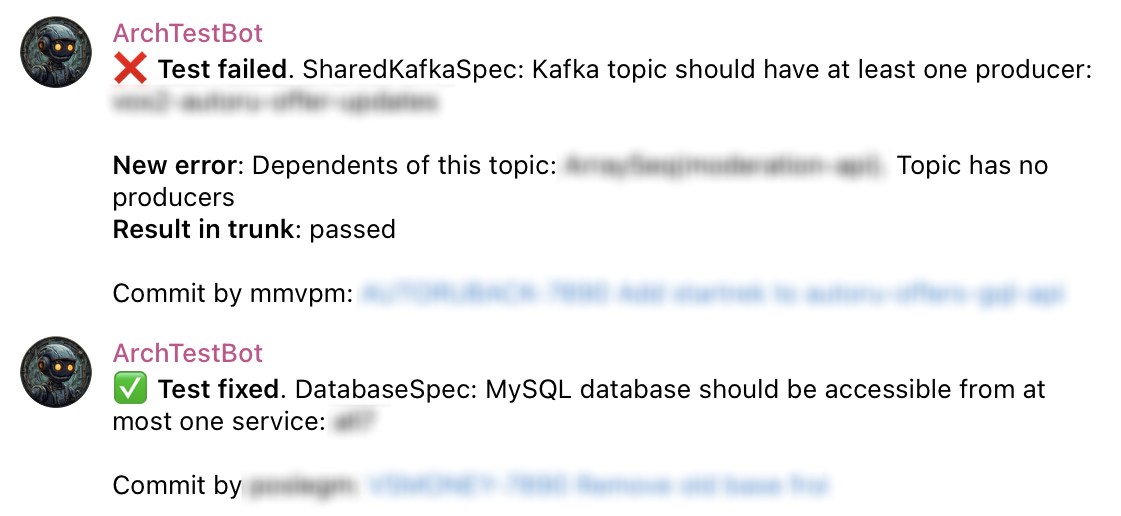
\includegraphics{images/telegram-notification-example.png}
}
\caption{
\label{telegram-notification-example} Пример уведомлений в Telegram.}
\end{flushleft}
\end{figure}


\end{document}
